\let\negmedspace\undefined
\let\negthickspace\undefined
\documentclass[journal]{IEEEtran}
\usepackage[a5paper, margin=10mm, onecolumn]{geometry}
\usepackage{tfrupee}
\usepackage{float}

\setlength{\headheight}{1cm}
\setlength{\headsep}{0mm}

\usepackage{gvv-book}
\usepackage{gvv}
\usepackage{cite}
\usepackage{amsmath,amssymb,amsfonts,amsthm}
\usepackage{algorithmic}
\usepackage{graphicx}
\usepackage{textcomp}
\usepackage{xcolor}
\usepackage{txfonts}
\usepackage{listings}
\usepackage{enumitem}
\usepackage{mathtools}
\usepackage{gensymb}
\usepackage{comment}
\usepackage[breaklinks=true]{hyperref}
\usepackage{tkz-euclide}
\usepackage[latin1]{inputenc}
\graphicspath{{figs/}}
\usepackage{color}
\usepackage{array}
\usepackage{longtable}
\usepackage{calc}
\usepackage{multirow}
\usepackage{hhline}
\usepackage{ifthen}
\usepackage{lscape}
\usepackage{circuitikz}

\begin{document}

\bibliographystyle{IEEEtran}
\vspace{3cm}

\title{4.3.10}
\author{EE25BTECH11007- Aniket}
\maketitle
{\let\newpage\relax\maketitle}

\setlength{\intextsep}{10pt}
\textbf{Question}:\\
Find the direction and normal vectors of the line $x - y = 2$.

\section*{Solution}
A line can be expressed in two forms:
\begin{equation}
\begin{pmatrix} x \\ y \end{pmatrix}
=
\begin{pmatrix} 0 \\ c \end{pmatrix}
+ x
\begin{pmatrix} 1 \\ m \end{pmatrix}
\label{eq:param}
\end{equation}
where $\begin{pmatrix} 1 \\ m \end{pmatrix}$ is the direction vector and $m$ is the slope.

\begin{equation}
\vec{n}^{\top}\,x = c
\label{eq:normal}
\end{equation}
where $\vec{n}$ is the normal vector of the line.

\begin{equation}
\vec{n}^{\top}
\begin{pmatrix} 1 \\ m \end{pmatrix}
= 0
\label{eq:orth}
\end{equation}

From $x - y = 2$ ,the slope is $m=1$. Hence, using \eqref{eq:param},
\begin{equation}
\begin{pmatrix} x \\ y \end{pmatrix}
=
\begin{pmatrix} 0 \\ -2 \end{pmatrix}
+ x
\begin{pmatrix} 1 \\ 1 \end{pmatrix}
\label{eq:param-inst}
\end{equation}

Let $\begin{pmatrix} x \\ y \end{pmatrix}$ be a normal vector. Then, from \eqref{eq:orth},
\begin{equation}
\begin{pmatrix} x \\ y \end{pmatrix}^{\!\top}
\begin{pmatrix} 1 \\ 1 \end{pmatrix}
= 0
\quad\Longrightarrow\quad
x + y = 0
\quad\Longrightarrow\quad
\begin{pmatrix} x \\ y \end{pmatrix}
=
\begin{pmatrix} 1 \\ -1 \end{pmatrix}
\label{eq:normal-inst}
\end{equation}

Line in normal form using \eqref{eq:normal} 
\[
\begin{pmatrix} 1 \\ -1 \end{pmatrix}^{\!\top}
\begin{pmatrix} x \\ y \end{pmatrix}
= 2
\]


Hence, the direction vector is
$\displaystyle \begin{pmatrix} 1 \\ 1 \end{pmatrix}$,
and the normal vector is
$\displaystyle \begin{pmatrix} 1 \\ -1 \end{pmatrix}$.

\begin{figure}[H]
    \centering
    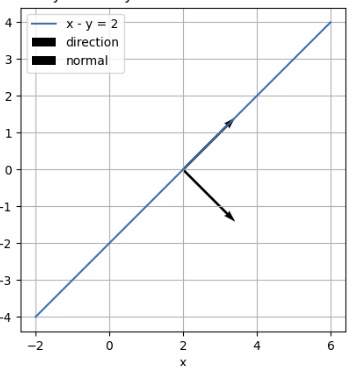
\includegraphics[width=\columnwidth]{figs/mg4plot.png}
\end{figure}

\end{document}
